\section{Abstract-""Syntax-""Tree (AST)}

Der Abstract-""Syntax-""Tree (AST) ist eine zentrale Datenstruktur im Programm, da jede Komponente mit ihr umgehen muss. Ableitungen und Assoziationen spiegeln direkt die Grammatik der WHILE-""Sprache wider. Da der AST von mehreren Komponenten mit unterschiedlichem Verhalten benutzt wird bietet sich hier das Visitor Entwurfsmuster (siehe Kapitel \ref{astvisitor_sec}) an.

\subsection{Visitor Entwurfsmuster}
\label{astvisitor_sec}
Das Visitor Pattern lagert die Operationen in externe Klassen (bspw. des Interpreters) aus. Somit lassen sich verschiedene, an den jeweiligen Verwendungszweck angepasste, Operationen auf dem selben AST ausführen. Jede Klasse erbt direkt oder indirekt durch die Ableitung der Klasse ASTNode die Funktion \texttt{accept ( visitor : ASTNodeVisitor )}. Dadurch lässt sich jede Klasse im Baum durch einen Visitor besuchen.
Ein geparsted Programm liegt durch die Assoziationen als Baum vor. Dieser lässt sich mithilfe der accept Methode traversieren. Jeder Knoten des Baums kann so erreicht werden und somit ist eine vollständige Abarbeitung des Programms gewährleistet. Der jeweilige Verwendungszweck ergibt sich durch die Benutzung verschiedener Visitors in der entsprechenden Komponente. 

\subsection{Klassenentwurf}
\subsubsection{abstract class ASTNode}
\label{astnode_class}
Grundsätzlich sind alle Klassen Ableitungen der Klasse ASTNode (siehe Abbildung \ref{ast_diag}). Hierdurch wird sicher gestellt, dass jede Klasse mittels der Methode \texttt{accept ( visitor : ASTNodeVisitor )} von einem Visitor besucht werden kann. Zusätzlich bietet diese Klasse Funktionen um Rückschlüsse (Position, Zeilennummer) auf den ursprünglichen Programmcode zu treffen.

\subsubsection{class Program}
Ein Objekt der Klasse Program stellt den Wurzelknoten eines geparsten Programms dar. Solch ein Program kann mehrere Funktionsdeklarationen (siehe Kapitel \ref{astfunctiondecl_class}) und maximal einen Block (siehe Kapitel \ref{astblock_class}), welcher als Main-Block des Programms fungiert, enthalten. Desweiteren kann ein Program eine Liste an Axiomen (siehe Abbildung \ref{ast_diag}) enthalten welche Aussagen über das Programm treffen.

\subsubsection{class FunctionDeclaration}
\label{astfunctiondecl_class}
In der Klasse FunctionDeclaration werden zu der jeweiligen Funktion, die Signatur (Name, Parameter, Rückgabetyp), der jeweilige Block (siehe Kapitel \ref{astblock_class}) und wahlweise Vor- und Nachbedingungen (siehe Abbildung \ref{ast_diag}) gespeichert.

\subsubsection{class Block}
\label{astblock_class}
Ein Block beinhaltet eine beliebige Anzahl an Statements (siehe Kapitel \ref{aststatement_class}).

\subsubsection{abstract class Statement}
\label{aststatement_class}
Diese Klasse dient dazu um die verschiedenen speziellen Statements (bspw. ReturnStatement, Assignment, VariableDeclaration, usw. siehe Abbildung \ref{ast_diag}) zu gruppieren.

\subsubsection{abstract class Expression}
\label{astexpr_class}
Ein Ausdruck spezialisiert sich in verschiedenen Klassen wie QuantifiedExpression, Literal, BinaryExpression, usw. (siehe Abbildung \ref{ast_diag}).

\begin{landscape}
\begin{figure}%
    \vspace{-2cm}%
    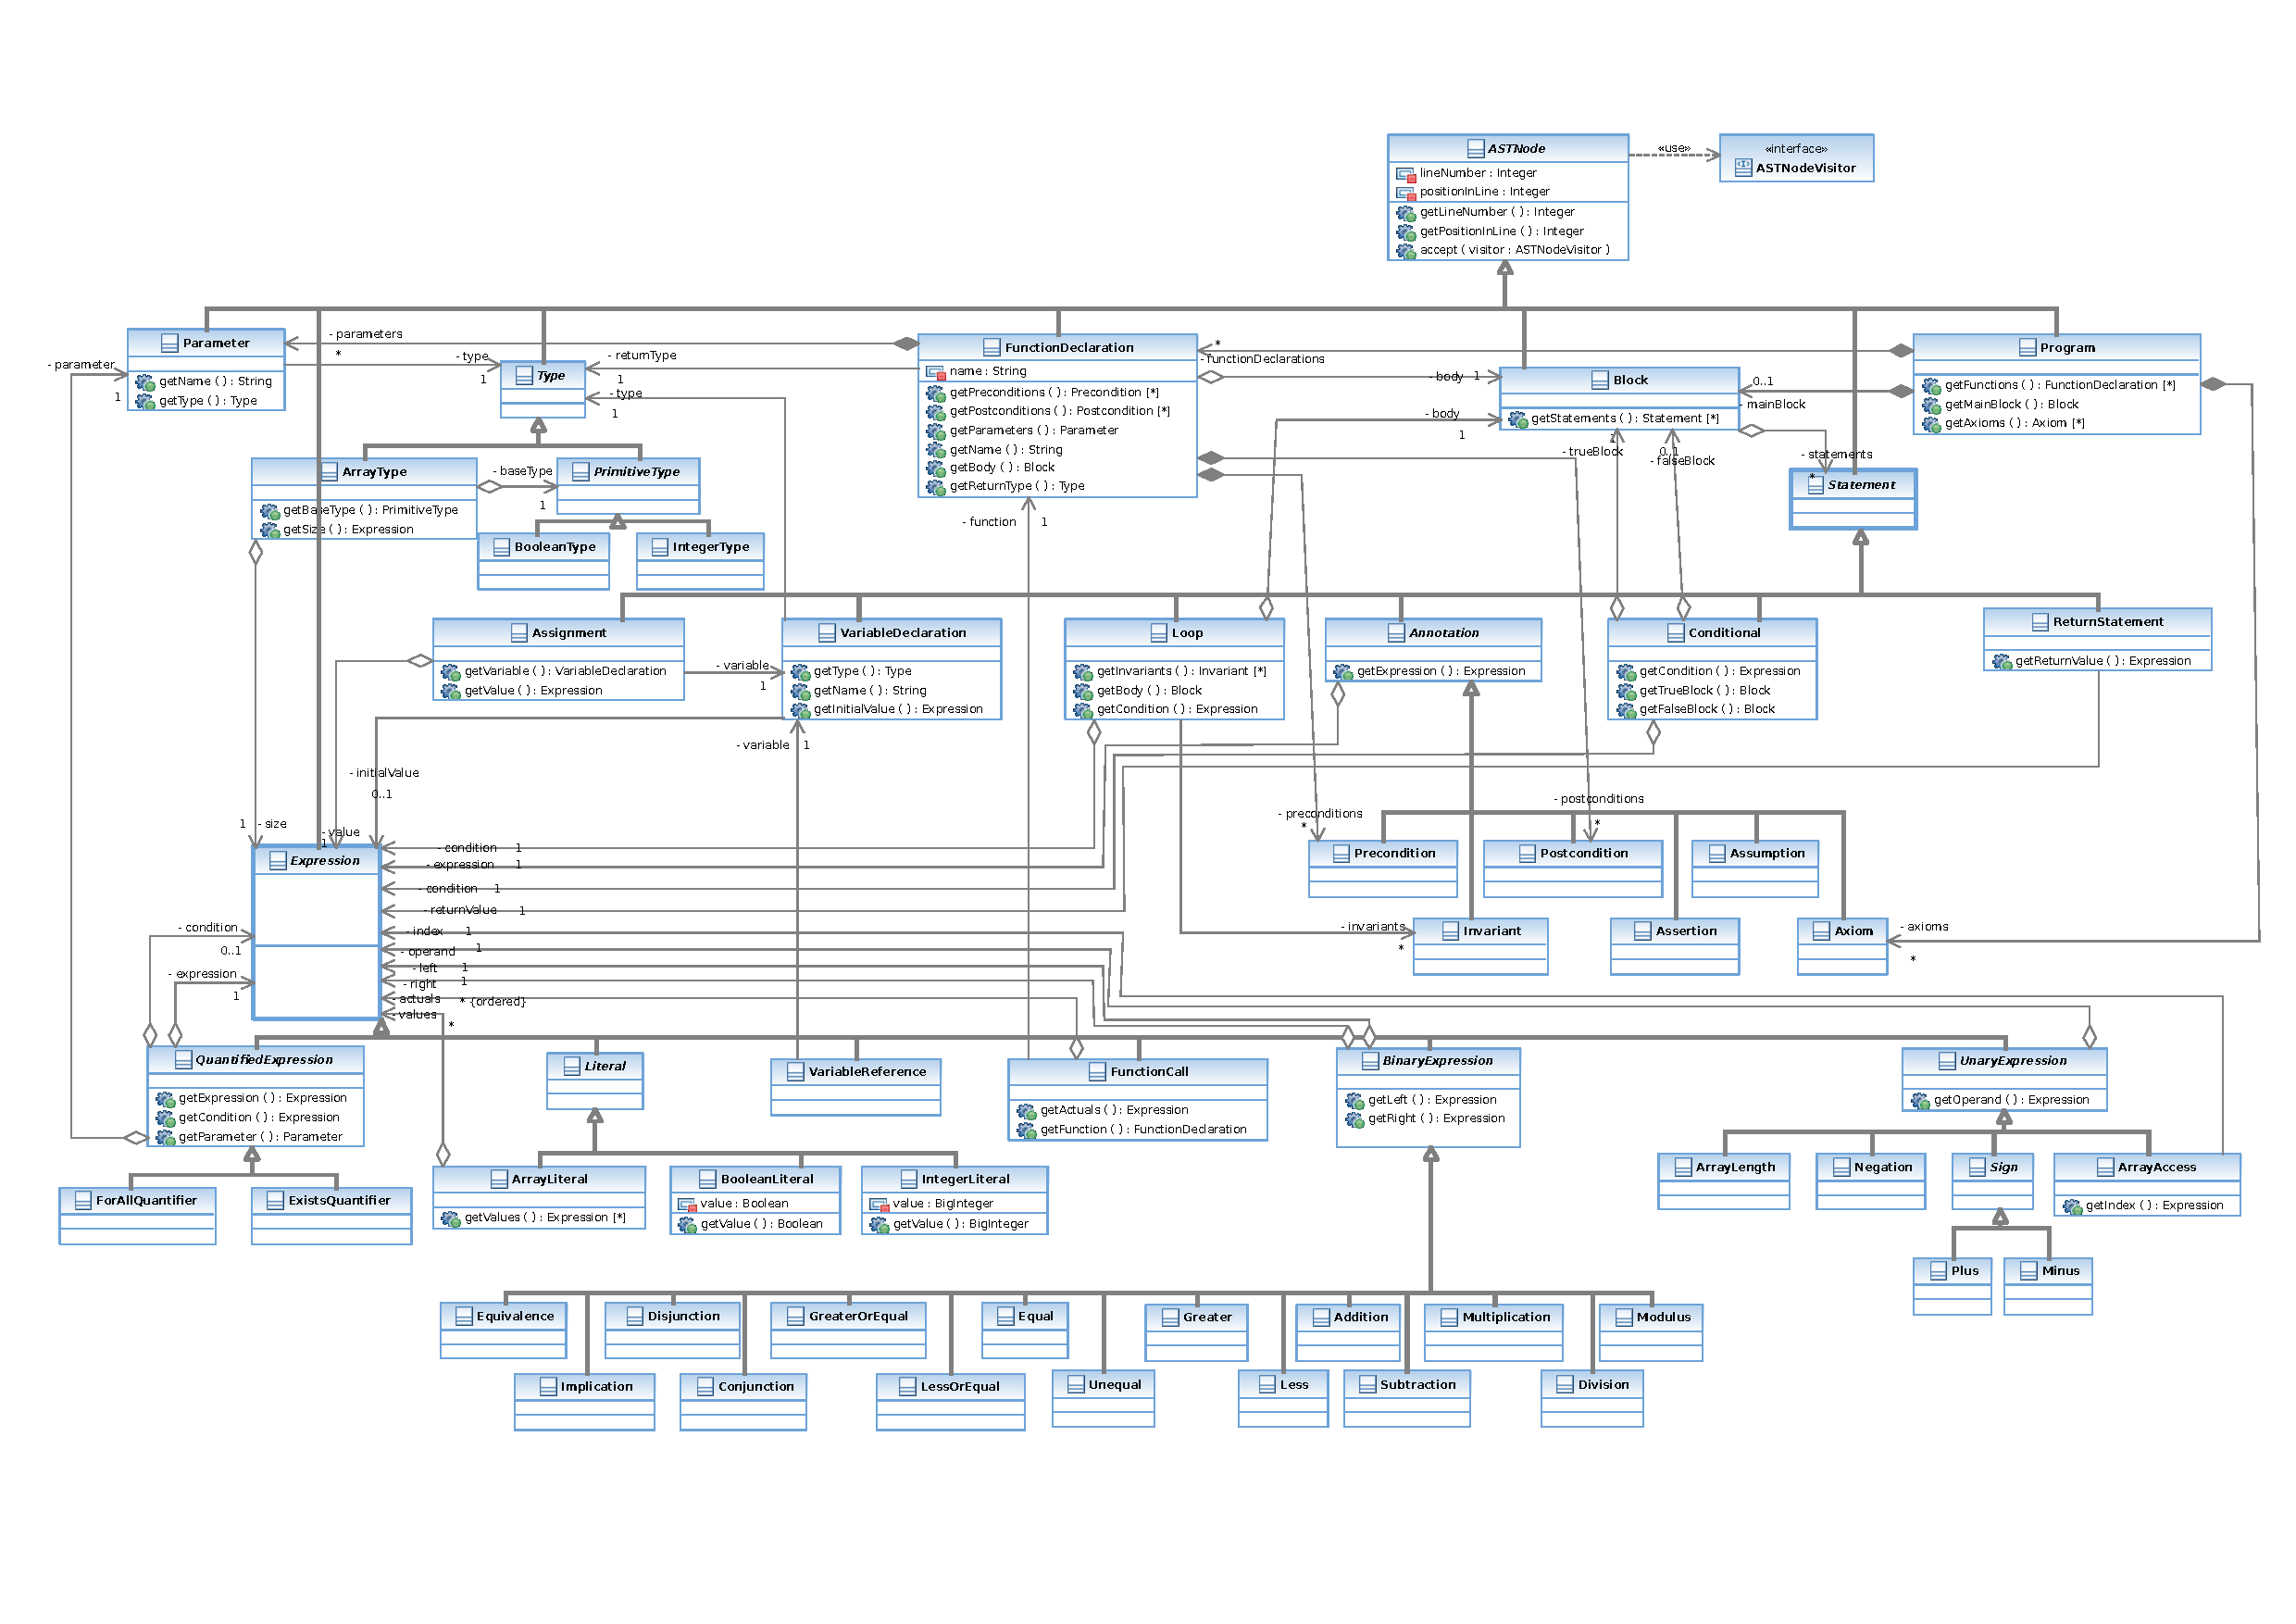
\includegraphics[height=\textheight]{diagrams/ast_component.pdf}

    \caption{Klassendiagramm des Abstract-""Syntax-""Trees mit den
    \type{Program}-""Bestandteilen \type{Statement} und
    \type{Expression} sowie der "`Besucher"'-""Klasse
    AST"-Node"-Visitor}

    \label{ast_diag}
\end{figure}%
\end{landscape}
